% latexmk -pdf pm2-model-derivation-reworked.tex && latexmk -c

\documentclass[10pt, a4paper]{article}

\usepackage[T1]{fontenc}
\usepackage[utf8]{inputenc}
\usepackage{mathtools}
\usepackage{amssymb}
\usepackage{bm}
\usepackage{physics}
\usepackage{amsthm}
\usepackage[margin=2.5cm]{geometry}
\usepackage{mymacros}
\usepackage{hyperref}
\usepackage{glossaries}
\usepackage{myacronyms}
\makenoidxglossaries
\newtheorem{remark}{Remark}

\title{Derivation of the four-state kite model\\ and explicit expression of the generalized accelerations}
\author{}
\date{}

\begin{document}
\maketitle

\section{Scope and notation}
\label{sec:scope}

This note derives, in one pass and without a symbolic solver, the explicit
second-order \gls{ode} governing the four-state \emph{point-mass} model of the
KEEP device: a generator drives an oscillating rigid arm; the arm tip
carries, through $n$ rigid lines of length $\ell$, a kite flying a
prescribed lemniscate on a cone (the kite is not attached to the arm
directly).
The state is $\bigl(\vq, \dq\bigr) \in
\R^4$ with generalized coordinates $\vq = (\alpha, \tau)$; the end result is a
closed formula for the generalized accelerations $\ddq \in \R^2$,
\eqref{eq:ddq-final} below, whose every entry is a function of $(\vq, \dq)$
and of the parameters listed here.  The model has two \gls{dof}; the
alternative five-state formulation with three algebraic loop-closure
constraints (a \gls{dae}) is described in \ref{sec:model10D}.

Throughout, all notation is introduced before use:
\begin{itemize}
    \item geometrical parameters: arm length $a$, line length $\ell$, with
    \begin{equation} \label{eq:ineq-l-a}
        \ell > a
    \end{equation}
    (in practice $\ell > 10$\,m and $a = 2$\,m);
    \item configuration variables (generalized coordinates) $\alpha, \tau$;
    \item generalized velocities $\dq = (\dot\alpha, \dot\tau)$ and
    accelerations $\ddq = (\ddot\alpha, \ddot\tau)$;
    \item other parameters: kite mass $m$, line mass
    $m_\ell = n \pi \ell \rho_\ell d_\ell$ ($n$ lines), arm inertia $I$,
    generator damping $b > 0$, aerodynamic and wind parameters
    (Section~\ref{sec:forces}).
\end{itemize}
Bold lowercase letters denote column vectors of $\R^3$; a hat denotes a unit
vector; $\vdot$ is the Euclidean scalar product; $e_1 = (1, 0)^\top \in
\R^2$.  Spherical coordinates of the kite position follow the physics
convention (ISO 80000-2): $r$ is the radius from the origin, $\theta$ the
polar angle from $\vu z$, $\phi$ the azimuthal angle from $\vu x$.
% note (r vs R): the kite radius is lowercase r throughout, ISO-style;
% src/PointMass4.jl still calls it R (compute_Rτ, variable R).

\section{Configuration and generalized coordinates}
\label{sec:configuration}

\subsection{Reference frame, arm and kite trajectory}

We fix a direct orthonormal frame $(O, \vu x, \vu y, \vu z)$ with $\vu x$
pointing downwind and $\vu z$ upward.  The arm rotates about $(O, \vu z)$;
its tip $A$ has position
\begin{equation}
    \vb a = \OA = a\,\ahat(\alpha),
    \qquad
    \ahat(\alpha) = \begin{pmatrix} \cos\alpha \\ \sin\alpha \\ 0 \end{pmatrix},
    \qquad \alpha \in [0, 2\pi).
\end{equation}

The kite $K$ is constrained to move on the cone with apex $O$ generated by
the lemniscate direction $\rhat(\tau)$,
\begin{equation}
    \OK = r\,\rhat(\tau),
    \qquad
    \rhat(\tau) = \begin{pmatrix}
        \sin\theta(\tau)\cos\phi(\tau) \\
        \sin\theta(\tau)\sin\phi(\tau) \\
        \cos\theta(\tau)
    \end{pmatrix},
    \qquad \tau \in [0, 2\pi),
\end{equation}
where the trajectory on the unit sphere is the figure eight
\begin{equation} \label{eq:lemniscate}
    \theta(\tau) = \theta_0 + \Delta\theta \sin(2\tau),
    \qquad
    \phi(\tau) = \phi_0 + \Delta\phi \sin(\tau),
\end{equation}
with mean polar angle $\theta_0$ and amplitudes $\Delta\theta$, $\Delta\phi$
satisfying $\theta_0 \pm \Delta\theta \subset (0, \pi)$ (the kite never flies
through the poles).

\subsection{Loop constraint and the radial coordinate}

The line joins $A$ to $K$, so $\AK = \OK - \OA$ and the constraint
$\norm{\AK} = \ell$ reads, with $p(\alpha, \tau) := \rhat \vdot \vb a$,
\begin{equation} \label{eq:loop}
    \norm{\OK - \vb a}^2 = \ell^2
    \quad\Longleftrightarrow\quad
    r^2 - 2pr + a^2 - \ell^2 = 0.
\end{equation}
Since $\rhat$ is a unit vector,
\begin{equation} \label{eq:p}
    p(\alpha, \tau)
    = a\,\ahat \vdot \rhat
    = a \sin\theta(\tau) \cos\bigl(\phi(\tau) - \alpha\bigr).
\end{equation}
Equation \eqref{eq:loop} has the two roots $p \pm \sqrt{p^2 + \ell^2 - a^2}$.
By \eqref{eq:ineq-l-a},
\begin{equation} \label{eq:Delta}
    \Delta(\alpha, \tau)
    := \sqrt{p^2 + \ell^2 - a^2}
    \;\ge\; \sqrt{\ell^2 - a^2}
    \;>\; 0,
\end{equation}
so the negative root satisfies $p - \Delta \le -\lvert p \rvert - \Delta < 0$
and only the positive root corresponds to $r > 0$ (kite above ground):
\begin{equation} \label{eq:R}
    r(\alpha, \tau) = p(\alpha, \tau) + \Delta(\alpha, \tau) > 0.
\end{equation}
In particular $r$ is a smooth function of $(\alpha, \tau)$: condition
\eqref{eq:ineq-l-a} is exactly what removes the square-root singularity of
the loop constraint.  The unit vector along the line is
\begin{equation} \label{eq:lhat}
    \lhat = \frac{\AK}{\ell}
    = \frac{r\,\rhat - a\,\ahat}{\ell}.
\end{equation}

Equations \eqref{eq:lemniscate} and \eqref{eq:R} show that the pair
$\vq = (\alpha, \tau)$ determines the full configuration of the system:
$\tau$ fixes the direction $\rhat$ of the kite on the cone, $\alpha$ fixes
the arm, and $r(\alpha, \tau)$ closes the loop.  We therefore choose
$\vq = (\alpha, \tau)$ as generalized coordinates; the state of the model is
$\bigl(\vq, \dq\bigr) \in \R^4$.

\section{Kinematics}
\label{sec:kinematics}

We collect every derivative of the map $\vq \mapsto \OK(\vq)$ needed below.
The time derivatives of the trajectory parameters \eqref{eq:lemniscate} are
\begin{equation} \label{eq:theta-phi-derivatives}
    \begin{aligned}
        \theta' &= 2\Delta\theta \cos(2\tau),
        &\qquad \theta'' &= -4\Delta\theta \sin(2\tau),\\
        \phi' &= \Delta\phi \cos(\tau),
        &\qquad \phi'' &= -\Delta\phi \sin(\tau),
    \end{aligned}
\end{equation}
where primes denote differentiation with respect to $\tau$.

\subsection[Derivatives of the unit vector r]{Derivatives of the unit vector $\rhat$}

Let $\eh_\theta = \partial \rhat / \partial\theta$ and
$\eh_\phi = (\sin\theta)^{-1} \partial \rhat / \partial\phi$ be the spherical
unit vectors,
\begin{equation}
    \eh_\theta = \begin{pmatrix}
        \cos\theta\cos\phi \\ \cos\theta\sin\phi \\ -\sin\theta
    \end{pmatrix},
    \qquad
    \eh_\phi = \begin{pmatrix} -\sin\phi \\ \cos\phi \\ 0 \end{pmatrix}.
\end{equation}
The first and second $\tau$-derivatives of $\rhat$ are
\begin{align}
    \rhat' &= \theta' \eh_\theta + \phi'\sin\theta \, \eh_\phi
    = \begin{pmatrix}
        \theta'\cos\theta\cos\phi - \phi'\sin\theta\sin\phi \\
        \theta'\cos\theta\sin\phi + \phi'\sin\theta\cos\phi \\
        -\theta'\sin\theta
    \end{pmatrix},
    \label{eq:rhat-prime}\\
    \rhat'' &= -\norm{\rhat'}^2 \rhat
    + \bigl( \theta'' - \phi'^2 \sin\theta\cos\theta \bigr) \eh_\theta
    + \bigl( \phi''\sin\theta + 2\theta'\phi'\cos\theta \bigr) \eh_\phi,
    \label{eq:rhat-second}
\end{align}
with
\begin{equation} \label{eq:rhat-prime-norm}
    \norm{\rhat'}^2 = \theta'^2 + \sin^2\!\theta\,\phi'^2.
\end{equation}
Because $\norm{\rhat} = 1$, the orthogonality relations
\begin{equation} \label{eq:rhat-ortho}
    \rhat \vdot \rhat' = 0,
    \qquad
    \rhat \vdot \rhat'' = -\norm{\rhat'}^2,
    \qquad
    \rhat' \vdot \rhat''
    = \theta'\theta'' + \phi'\phi''\sin^2\!\theta
    + \theta'\phi'^2\sin\theta\cos\theta
\end{equation}
follow by differentiating once and twice; they are used in
Section~\ref{sec:assembly}.  For $\Delta\theta, \Delta\phi \ne 0$, the
quantities $\theta'$ and $\phi'$ never vanish simultaneously
($\cos 2\tau$ and $\cos\tau$ have no common zero), so
$\norm{\rhat'}^2 > 0$ along the whole lemniscate.

\subsection[Derivatives of p and r]{Derivatives of $p$ and $r$}

Write $\psi := \phi(\tau) - \alpha$, so that $p = a\sin\theta\cos\psi$ and,
at fixed $\alpha$, $\psi' = \phi'$.  The first derivatives of $p$ are
\begin{align}
    p_\alpha &= a \sin\theta \sin\psi,
    \label{eq:p-alpha}\\
    p_\tau &= a \bigl( \theta'\cos\theta\cos\psi
    - \phi'\sin\theta\sin\psi \bigr),
    \label{eq:p-tau}
\end{align}
and the second derivatives are
\begin{align}
    p_{\alpha\alpha} &= -a\sin\theta\cos\psi = -p,
    \label{eq:p-aa}\\
    p_{\alpha\tau} &= a \bigl( \theta'\cos\theta\sin\psi
    + \phi'\sin\theta\cos\psi \bigr),
    \label{eq:p-at}\\
    p_{\tau\tau} &= a \Bigl(
    \bigl( \theta''\cos\theta - (\theta'^2 + \phi'^2)\sin\theta \bigr)\cos\psi
    - 2\theta'\phi'\cos\theta\sin\psi
    - \phi''\sin\theta\sin\psi
    \Bigr).
    \label{eq:p-tt}
\end{align}
From \eqref{eq:Delta}--\eqref{eq:R} we obtain, by the chain rule,
\begin{equation} \label{eq:R-derivatives}
    \frac{\partial r}{\partial p} = \frac{r}{\Delta},
    \qquad
    \frac{\partial^2 r}{\partial p^2} = \frac{\ell^2 - a^2}{\Delta^3},
\end{equation}
hence
\begin{equation} \label{eq:R-grad}
    r_\alpha = \frac{r}{\Delta}\, p_\alpha,
    \qquad
    r_\tau = \frac{r}{\Delta}\, p_\tau,
\end{equation}
and the Hessian of $r$ splits as
\begin{equation} \label{eq:R-hessian}
    H_r
    := \begin{pmatrix} r_{\alpha\alpha} & r_{\alpha\tau} \\
        r_{\alpha\tau} & r_{\tau\tau} \end{pmatrix}
    = \frac{r}{\Delta} H_p
    + \frac{\ell^2 - a^2}{\Delta^3}
    \begin{pmatrix} p_\alpha^2 & p_\alpha p_\tau \\
        p_\alpha p_\tau & p_\tau^2 \end{pmatrix},
    \qquad
    H_p = \begin{pmatrix}
        p_{\alpha\alpha} & p_{\alpha\tau} \\
        p_{\alpha\tau} & p_{\tau\tau}
    \end{pmatrix}.
\end{equation}
All entries of $H_r$ are explicit in $(\vq)$ through
\eqref{eq:p-alpha}--\eqref{eq:p-tt}.

\subsection{Velocity and acceleration of the kite}

Introduce the intermediate coordinate $w := (r, \tau)^\top = \chi(\vq)$.
Throughout this section, $\operatorname{D}f$ denotes the derivative
(Jacobian) of a map $f$ and $\operatorname{D}^2f(x)(v, w)$ its second
derivative bilinear form.  Here
\begin{equation} \label{eq:chi}
    J_\chi(\vq) = \operatorname{D}\chi(\vq)
    = \begin{pmatrix} r_\alpha & r_\tau \\ 0 & 1 \end{pmatrix},
    \qquad
    \operatorname{D}^2\chi(\vq)(\dq, \dq)
    = \begin{pmatrix} \dq^\top H_r \dq \\ 0 \end{pmatrix}.
\end{equation}
As a function of $w$, the position $\OK = r\rhat(\tau)$ has Jacobian
\begin{equation} \label{eq:J-OK}
    J_{\OK}(w)
    := \frac{\partial \OK}{\partial (r, \tau)}
    = \begin{pmatrix} \rhat & r\,\rhat' \end{pmatrix}
    \in \R^{3\times 2},
    \qquad
    J_{\OK}^\top J_{\OK}
    = \operatorname{diag}\bigl(1,\; r^2\norm{\rhat'}^2\bigr),
\end{equation}
where the diagonal structure again uses $\rhat \vdot \rhat' = 0$; and the
second derivative in direction $(\dot r, \dot\tau)$ is
\begin{equation} \label{eq:D2-OK}
    \operatorname{D}^2\OK(w)\bigl((\dot r, \dot\tau), (\dot r, \dot\tau)\bigr)
    = 2\dot r\,\dot\tau\,\rhat' + r\,\dot\tau^{\,2}\,\rhat'',
\end{equation}
since $\partial^2\OK/\partial r^2 = 0$,
$\partial^2\OK/\partial r\partial\tau = \rhat'$ and
$\partial^2\OK/\partial\tau^2 = r\rhat''$.

Along any trajectory $t \mapsto \vq(t)$, the intermediate coordinate
$w(t) = \chi(\vq(t))$ satisfies, by the chain rule applied twice,
\begin{equation}
    \dot w = J_\chi \dq,
    \qquad
    \ddot w = J_\chi \ddq
    + \operatorname{D}^2\chi(\vq)(\dq, \dq),
\end{equation}
the second term being the acceleration of the reparametrization $\chi$ at
fixed velocity $\dq$.  Applying the same rule to the composition
$\vq \mapsto \chi(\vq) \mapsto \OK$, i.e.\ differentiating
$\OK\bigl(\chi(\vq(t))\bigr)$ twice with respect to time, gives
\begin{equation}
    \ddot{\OK}
    = J_{\OK} \, \ddot w
    + \operatorname{D}^2\OK(w)\bigl(\dot w, \dot w\bigr)
    = J(\vq)\, \ddq + \vb a_0(\vq, \dq),
\end{equation}
with the $3\times 2$ configuration Jacobian
% note (symbol rename): D(q) renamed to J(q) = J_OK J_chi after review --
% bare D clashed with the derivative operators D, D^2; J matches the
% J_OK, J_chi family.
\begin{equation} \label{eq:D}
    J(\vq)
    := J_{\OK}\, J_\chi
    = \frac{\partial \OK}{\partial \vq}
    = \begin{pmatrix} r_\alpha\,\rhat & r_\tau\,\rhat + r\,\rhat' \end{pmatrix}
\end{equation}
and the bias acceleration (centripetal/Coriolis terms, independent of $\ddq$)
\begin{equation} \label{eq:a0}
    \vb a_0(\vq, \dq)
    = \bigl( \dq^\top H_r \dq \bigr)\, \rhat
    + 2\dot r\,\dot\tau\,\rhat'
    + r\,\dot\tau^{\,2}\,\rhat'',
    \qquad
    \dot r = r_\alpha\dot\alpha + r_\tau\dot\tau.
\end{equation}
The two columns of the matrix $J(\vq)$ are the Cartesian vectors
$\partial\OK/\partial\alpha$ and $\partial\OK/\partial\tau$, elements of
$\R^3$, so $J(\vq)\,\dq$ is an ordinary velocity in $(x, y, z)$; the
kite velocity, needed for the aerodynamic forces, is
\begin{equation} \label{eq:velocity}
    \dot{\OK} = J(\vq)\,\dq \in \R^3.
\end{equation}
For reference, the scalar products of $\vb a_0$ with the columns of
$J_{\OK}$, which reappear in Section~\ref{sec:assembly}, reduce using
\eqref{eq:rhat-ortho} to
\begin{equation} \label{eq:a0-projections}
    \begin{aligned}
        \rhat \vdot \vb a_0
        &= \dq^\top H_r \dq - r\,\dot\tau^{\,2}\norm{\rhat'}^2,\\
        r\,\rhat' \vdot \vb a_0
        &= 2r\,\dot r\,\dot\tau\,\norm{\rhat'}^2
        + r^2\,\dot\tau^{\,2}\,(\rhat' \vdot \rhat'').
    \end{aligned}
\end{equation}

\section{Forces}
\label{sec:forces}

The kite of mass $m$ is subject to gravity, to the aerodynamic resultant and
to the line tension; an unknown reaction $\vb F_c$ accounts for the cone.
All forces apply at $K$; all moments apply to the arm.

\subsection{Gravity}

With $m_g := m + m_\ell / 2$ (the kite lifts half of the lines),
\begin{equation} \label{eq:f-grav}
    \vb F_g = -m_g\, g\,\vu z,
    \qquad
    m_\ell = n \pi \ell \rho_\ell d_\ell.
\end{equation}
In particular
\begin{equation} \label{eq:f-grav-projections}
    \rhat \vdot \vb F_g = -m_g\, g \cos\theta,
    \qquad
    r\,\rhat' \vdot \vb F_g = m_g\, g\, r\,\theta'\sin\theta,
\end{equation}
using $\rhat_z = \cos\theta$ and $\rhat'_z = -\theta'\sin\theta$.

\subsection{Apparent wind and aerodynamic forces}

The wind profile follows the one-seventh power law; since $\vu x$ points
downwind,
\begin{equation} \label{eq:wind}
    \vb w(z) = w_{\mathrm{ref}}
    \Bigl( \frac{z}{z_{\mathrm{ref}}} \Bigr)^{1/7} \vu x,
    \qquad
    z = \rhat_z r = r\cos\theta.
\end{equation}
The apparent wind felt by the kite is
\begin{equation} \label{eq:apparent-wind}
    \vb w_a = \vb w(z) - \dot{\OK}
    = \vb w(z) - J\,\dq.
\end{equation}
Lift and drag of the kite are
\begin{equation} \label{eq:lift-drag}
    L = \tfrac{1}{2}\,\rho_a S C_L \norm{\vb w_a}^2,
    \qquad
    D_{\mathrm{drag}} = \frac{L}{f},
\end{equation}
$f = L/D$ being the lift-to-drag ratio.  The drag of the $n$ lines follows
from strip theory: the element $[\lambda, \lambda + \dd\lambda]$ of one
line sees the apparent wind $\vb w_{a,\ell}(\lambda)$ and presents the
area component perpendicular to both the line and the wind,
$d_\ell \bigl(1 - (\lhat \vdot \vu w_{a,\ell})^2\bigr) \dd\lambda$, so
\begin{equation} \label{eq:line-drag-integral}
    \tilde{\vb D}_\ell
    = \frac{1}{2}\, n \, \rho_a C_{D,\ell} \, d_\ell
    \int_0^\ell
    \bigl(1 - (\lhat \vdot \vu w_{a,\ell})^2\bigr)\,
    \norm{\vb w_{a,\ell}(\lambda)}^2\,
    \vb w_{a,\ell}(\lambda)\, \dd\lambda.
\end{equation}
% note (line drag): direction of the result taken along k_b; the source
% notes wavered between k_b and w_a -- k_b keeps F_a = L k_t + (D+Dt) k_b.
We evaluate \eqref{eq:line-drag-integral} under three approximations:
\begin{enumerate}
    \item the speed of the attachment point $A$ is negligible and the
    wind profile is nearly linear along the line, so
    $\vb w_{a,\ell}(\lambda) \approx \tfrac{\lambda}{\ell} \vb w_a$;
    \item the apparent wind is perpendicular to the lines,
    $1 - (\lhat \vdot \vu w_{a,\ell})^2 \approx 1$;
    \item the direction of the elementary drag is that of the kite drag,
    along $\vu k_b$.
\end{enumerate}
Then, with $\xi = \lambda/\ell$,
\begin{equation}
    \tilde D_\ell
    = \frac{1}{2}\, n \ell d_\ell \rho_a C_{D,\ell}
    \norm{\vb w_a}^2 \int_0^1 \xi^2 \dd\xi
    = \frac{1}{6}\, n \ell d_\ell \rho_a C_{D,\ell}
    \norm{\vb w_a}^2.
\end{equation}
The orientation of the kite is fixed by
assuming zero angle of incidence: the chord is aligned with $\vb w_a$ and
the leading edge is perpendicular to the lines, i.e.
\begin{equation} \label{eq:aero-frame}
    \vu k_b = \frac{\vb w_a}{\norm{\vb w_a}},
    \qquad
    \vu k_r = \frac{\lhat \times \vu k_b}{\norm{\lhat \times \vu k_b}},
    \qquad
    \vu k_t = \vu k_b \times \vu k_r,
\end{equation}
and the total aerodynamic force is
\begin{equation} \label{eq:f-aero}
    \vb F_a = L\,\vu k_t
    + \bigl( D_{\mathrm{drag}} + \tilde D_\ell \bigr) \vu k_b.
\end{equation}
The line drag is aligned with the kite drag direction; its reaction on
the arm is neglected.
By \eqref{eq:velocity} and \eqref{eq:wind}--\eqref{eq:apparent-wind}, the
force $\vb F_a$ depends on
$(\vq, \dq)$ only, \emph{not} on $\ddq$.  Regularity requires
$\vb w_a \ne 0$ and $\lhat \times \vu k_b \ne 0$ (apparent wind not parallel
to the lines), which hold along the trajectories of interest.

\subsection{Line tension from the arm balance}

The arm rotates about $(O, \vu z)$ with inertia $I$; the generator applies
the resistive torque $T_{\mathrm{gen}}(\dot\alpha) = -b\dot\alpha$, $b > 0$.
Let $S \ge 0$ be the tension magnitude, i.e.\ the lines pull the kite
towards $A$ with force $-S\lhat$ and pull the arm tip towards $K$ with force
$S\lhat$.  The moment of the latter about $(O, \vu z)$ is
\begin{equation}
    \bigl( \vb a \times S\lhat \bigr) \vdot \vu z
    = S\,a\,\lhat \vdot (\vu z \times \ahat)
    = S\,\mu,
\end{equation}
and the scalar moment arm $\mu$ simplifies using \eqref{eq:lhat} and
$\ahat \vdot (\vu z \times \ahat) = 0$:
\begin{equation} \label{eq:mu}
    \mu(\vq)
    := a\,\lhat \vdot (\vu z \times \ahat)
    = \frac{a r}{\ell}\, \rhat \vdot (\vu z \times \ahat)
    = \frac{a r}{\ell}\, \sin\theta \sin(\phi - \alpha).
\end{equation}
Newton's second law for the arm,
\begin{equation} \label{eq:arm-balance}
    I\,\ddot\alpha = S\,\mu + T_{\mathrm{gen}}(\dot\alpha)
    = S\,\mu - b\,\dot\alpha,
\end{equation}
is linear in $S$ and yields
\begin{equation} \label{eq:tension-magnitude}
    S = \frac{I\,\ddot\alpha + b\,\dot\alpha}{\mu},
    \qquad\text{hence the force on the kite}\qquad
    \vb F_\ell = -S\,\lhat
    = -\frac{I\,\ddot\alpha + b\,\dot\alpha}{\mu}\,\lhat.
\end{equation}
Separating the part that carries $\ddq$, with $\kappa \vcentcolon= I/\mu$,
\begin{equation} \label{eq:f-lines}
    \vb F_\ell
    = -\kappa\,\lhat\, e_1^\top \ddq
    - \frac{b\,\dot\alpha}{\mu}\,\lhat.
\end{equation}
\begin{remark}
    The model requires $\mu \ne 0$; $\mu$ vanishes when the lines lie in
    the vertical half-plane of the arm.  Remark~\ref{rem:regularity} in
    Section~\ref{sec:explicit-ddq} develops what this means in practice.
\end{remark}

\subsection{Newton's law and the cone reaction}

Newton's second law applied to the kite reads
\begin{equation} \label{eq:newton-kite}
    m\,\ddot{\OK}
    = \vb F_a + \vb F_g + \vb F_\ell + \vb F_c ,
\end{equation}
where the fictitious force $\vb F_c$ plays the role of the rail in a
railway analogy: it keeps the kite on the prescribed cone without doing work
along the motion on the cone.  The tangent space of the cone
$\mathcal{C} = \{ \rho\,\rhat(\tau') \mid \rho > 0,\ \tau' \in [0, 2\pi) \}$ at
the configuration is spanned by $\rhat$ ($\partial/\partial r$) and
$r\rhat'$ ($\partial/\partial\tau$), i.e.\ exactly by the columns of
$J_{\OK}$ \eqref{eq:J-OK}.  Sliding without friction on the cone means
d'Alembert's principle
\begin{equation} \label{eq:cone-dalembert}
    J_{\OK}^\top\, \vb F_c = 0
    \qquad\Longleftrightarrow\qquad
    \vb F_c \vdot \rhat = 0
    \quad\text{and}\quad
    \vb F_c \vdot (r\rhat') = 0.
\end{equation}

\section{Assembly of the equations of motion}
\label{sec:assembly}

Insert the kinematic identity $\ddot{\OK} = J\ddq + \vb a_0$
\eqref{eq:D}--\eqref{eq:a0} and the tension \eqref{eq:f-lines} into
Newton's law \eqref{eq:newton-kite} and isolate $\vb F_c$:
\begin{equation} \label{eq:F_c}
    \vb F_c
    = \underbrace{\bigl[ m\,J + \kappa\,\lhat\, e_1^\top \bigr]}_{3\times 2}
    \ddq
    + \underbrace{\Bigl[ m\,\vb a_0 - \vb F_a - \vb F_g
    + \frac{b\,\dot\alpha}{\mu}\,\lhat \Bigr]}_{3\times 1}.
\end{equation}
Both brackets depend on $(\vq, \dq)$ only.  Projecting with
$J_{\OK}^\top$ and imposing \eqref{eq:cone-dalembert} eliminates $\vb F_c$
and gives a $2\times 2$ linear system for $\ddq$,
\begin{equation} \label{eq:eom-matrix}
    \boxed{\; M(\vq)\,\ddq = \vb h(\vq, \dq) \;}
\end{equation}
with
\begin{equation} \label{eq:M-h-def}
    M(\vq)
    = J_{\OK}^\top \bigl[ m\,J + \kappa\,\lhat\, e_1^\top \bigr],
    \qquad
    \vb h(\vq, \dq)
    = -J_{\OK}^\top \Bigl[ m\,\vb a_0 - \vb F_a - \vb F_g
    + \frac{b\,\dot\alpha}{\mu}\,\lhat \Bigr].
\end{equation}
We now make both sides fully explicit.  Three short computations suffice.

\noindent\textbf{(i) Kinematic block.}
Using $J = J_{\OK} J_\chi$ \eqref{eq:D} and the diagonal metric
\eqref{eq:J-OK},
\begin{equation}
    m\,J_{\OK}^\top J
    = m\, \operatorname{diag}\bigl(1,\; r^2\norm{\rhat'}^2\bigr)
    \begin{pmatrix} r_\alpha & r_\tau \\ 0 & 1 \end{pmatrix}
    = m \begin{pmatrix}
        r_\alpha & r_\tau \\
        0 & r^2\bigl( \theta'^2 + \sin^2\!\theta\,\phi'^2 \bigr)
    \end{pmatrix}.
\end{equation}

\noindent\textbf{(ii) Tension block.}
From \eqref{eq:lhat} and \eqref{eq:R-grad},
\begin{equation} \label{eq:lhat-projections}
    \rhat \vdot \lhat = \frac{r - a\,\ahat\vdot\rhat}{\ell}
    = \frac{r - p}{\ell}
    = \frac{\Delta}{\ell},
    \qquad
    r\,\rhat' \vdot \lhat
    = -\frac{a r}{\ell}\, \rhat'\vdot\ahat
    = -\frac{\Delta}{\ell}\, r_\tau ,
\end{equation}
because $\rhat'\vdot\ahat = p_\tau/a$ by \eqref{eq:p-tau} and
$r_\tau = (r/\Delta) p_\tau$.  Hence
\begin{equation}
    \kappa\, J_{\OK}^\top \lhat\, e_1^\top
    = \frac{\kappa\Delta}{\ell}
    \begin{pmatrix} 1 \\ -r_\tau \end{pmatrix}
    \begin{pmatrix} 1 & 0 \end{pmatrix}
    = \frac{\kappa\Delta}{\ell}
    \begin{pmatrix} 1 & 0 \\ -r_\tau & 0 \end{pmatrix}.
\end{equation}

\noindent\textbf{(iii) Right-hand side.}
Projecting the bias acceleration with \eqref{eq:a0-projections}, gravity
with \eqref{eq:f-grav-projections} and the damping tension with
\eqref{eq:lhat-projections},
\begin{equation} \label{eq:h-explicit}
    \begin{aligned}
        h_1 &= -m \Bigl( \dq^\top H_r \dq
        - r\,\dot\tau^{\,2} \norm{\rhat'}^2 \Bigr)
        + \rhat \vdot \vb F_a
        - m_g\, g \cos\theta
        - \frac{b\,\dot\alpha\,\Delta}{\mu\,\ell}, \\
        h_2 &= -2m\,r\,\dot r\,\dot\tau\,\norm{\rhat'}^2
        - m\,r^2\,\dot\tau^{\,2}\,(\rhat'\vdot\rhat'')
        + r\,\rhat' \vdot \vb F_a
        + m_g\, g\, r\,\theta'\sin\theta
        + \frac{b\,\dot\alpha\,\Delta\,r_\tau}{\mu\,\ell}.
    \end{aligned}
\end{equation}

Collecting (i)--(iii), the mass matrix is the explicit $2\times 2$ matrix
\begin{equation} \label{eq:M-explicit}
    M(\vq)
    = \begin{pmatrix}
        m\,r_\alpha + \dfrac{\kappa\Delta}{\ell}
        & m\,r_\tau \\[2mm]
        -\dfrac{\kappa\Delta}{\ell}\,r_\tau
        & m\,r^2\bigl( \theta'^2 + \sin^2\!\theta\,\phi'^2 \bigr)
    \end{pmatrix},
    \qquad
    \kappa = \frac{I}{\mu},
\end{equation}
with $\vb h$ given by \eqref{eq:h-explicit}; every entry is a function of
$\vq$ (through \eqref{eq:theta-phi-derivatives},
\eqref{eq:p-alpha}--\eqref{eq:R-hessian}, \eqref{eq:Delta},
\eqref{eq:mu}) and, for $h_1, h_2$, of $\dq$ (through $H_r\dq$-terms,
$\dot r$, $\vb F_a(\vq, \dq)$).

\section{Explicit solution for the generalized accelerations}
\label{sec:explicit-ddq}

System \eqref{eq:eom-matrix} is linear with $2\times 2$ coefficient matrix,
so it is solved by Cramer's rule.  Its determinant is
\begin{equation} \label{eq:det-M}
    \det M
    = m\,r^2\bigl( \theta'^2 + \sin^2\!\theta\,\phi'^2 \bigr)
    \Bigl( m\,r_\alpha + \frac{\kappa\Delta}{\ell} \Bigr)
    + m\,\frac{\kappa\Delta}{\ell}\,r_\tau^2 ,
\end{equation}
and the explicit expression of the generalized accelerations is
\begin{equation} \label{eq:ddq-final}
    \ddq
    = \frac{1}{\det M}
    \begin{pmatrix}
        M_{22}\, h_1 - M_{12}\, h_2 \\[1mm]
        M_{11}\, h_2 - M_{21}\, h_1
    \end{pmatrix}
    = \frac{1}{\det M}
    \begin{pmatrix}
        m r^2\bigl( \theta'^2 + \sin^2\!\theta\,\phi'^2 \bigr)\, h_1
        - m r_\tau\, h_2 \\[1mm]
        \Bigl( m r_\alpha + \dfrac{\kappa\Delta}{\ell} \Bigr) h_2
        + \dfrac{\kappa\Delta}{\ell}\,r_\tau\, h_1
    \end{pmatrix},
\end{equation}
where $h_1, h_2$ are given by \eqref{eq:h-explicit},
$M_{ij}$ by \eqref{eq:M-explicit}, and all elementary ingredients are
listed in Sections~\ref{sec:configuration}--\ref{sec:forces}.
Thus $\ddq = F(\vq, \dq)$ is an elementary function of the state: no
linear system, no symbolic output and no algebraic constraint is left to
satisfy.

\begin{remark}[Regularity]
    \label{rem:regularity}
    \begin{enumerate}
        \item $\ell > a$ \eqref{eq:ineq-l-a} guarantees $\Delta > 0$
        \eqref{eq:Delta}, hence a smooth $r$ and bounded $M_{ij}$.
        \item \emph{The condition $\mu \ne 0$.}
        Geometrically $\mu = \vu z \vdot (\vb a \times \lhat)$ is the signed
        lever arm of the line tension about $(O, \vu z)$: its moment is
        $S\mu$.  It vanishes exactly when the kite, the arm tip and the
        $z$-axis are coplanar, $\phi(\tau) \equiv \alpha \bmod \pi$.

        Along a trajectory this happens at isolated times and, generically,
        \emph{transversally}: at a crossing $t_\star$,
        \begin{equation*}
            \frac{\mathrm d}{\mathrm dt}\bigl(\phi(\tau) - \alpha\bigr)
            \Big|_{t_\star}
            = \phi'\dot\tau - \dot\alpha \ne 0
            \qquad\Longrightarrow\qquad
            \lvert\mu(t)\rvert \approx
            \lvert\dot\mu(t_\star)\rvert\, \lvert t - t_\star\rvert .
        \end{equation*}
        The trajectory thus leaves every neighbourhood of the singular set
        in finite time: the window where the ill-conditioned regime of
        item 3 is visited has width
        $\mathcal{O}(1/\lvert\dot\mu(t_\star)\rvert)$.  What transversality
        excludes is a \emph{grazing} contact, $\phi'\dot\tau = \dot\alpha$
        at $\phi = \alpha$, where $\mu$ would linger near zero.  On the
        monitored cycle both crossings are transversal, with measured
        $\phi'\dot\tau - \dot\alpha = -2.0$ and $+2.0$
        ($\lvert\dot\mu\rvert \approx 3.6$\,m/s).

        Exactly on the set evaluation must be avoided anyway: in floating
        point $\sin(\phi - \alpha) = 0$ makes $\kappa = I/\mu$ a
        \texttt{NaN}, so the implementation starts the lemniscate at
        $\tau_0 = 10^{-10}$ rather than $0$ (\texttt{TAU0} in
        \texttt{src/KEEP.jl}).  The model also requires $S \ge 0$ (lines
        cannot push); on the monitored cycle $S \in [2.8, 9.5]$\,kN.  The
        singularity itself is removable, as item 3 shows.
        \item \emph{Conditioning of $M$; the singularity is removable.}
        The tension adds a rank-one term to the kinetic block: collecting
        \eqref{eq:arm-balance}--\eqref{eq:f-lines},
        \begin{equation*}
            M = M_{\mathrm{kin}} + \mu^{-1} I\, \vb u\, e_1^\top,
            \qquad
            \vb h = \vb h_0 - \mu^{-1}\, b\dot\alpha\, \vb u,
        \end{equation*}
        with $\vb u = (\Delta/\ell)\,(1, -r_\tau)^\top$,
        $M_{\mathrm{kin}} = m\,\operatorname{diag}\bigl(1,
        r^2\norm{\rhat'}^2\bigr) J_\chi$ and
        $\vb h_0 = m\vb a_0 - \vb F_a - \vb F_g$.  The factor $\mu^{-1}$
        is an artefact of solving the arm balance for the tension first,
        $S = (I\ddot\alpha + b\dot\alpha)/\mu$
        \eqref{eq:tension-magnitude}, which bakes it into $\vb F_\ell$
        and hence into $M$ and $\vb h$.  Consequently
        $\norm{M}_2 = \Theta(1/\lvert\mu\rvert)$ as $\mu \to 0$, and if
        $M_{\mathrm{kin}}$ stays definite then
        $\operatorname{cond}_2 M = \Theta(1/\lvert\mu\rvert)$ at the
        crossings.  Sherman--Morrison removes the singularity: for
        $w := e_1^\top M_{\mathrm{kin}}^{-1} \vb u \ne 0$,
        \begin{equation*}
            \ddq
            = M_{\mathrm{kin}}^{-1} \vb h_0
            - \frac{I\, e_1^\top M_{\mathrm{kin}}^{-1} \vb h_0
            + b\dot\alpha}{\mu + I\,w}\,
            M_{\mathrm{kin}}^{-1} \vb u ,
        \end{equation*}
        whose right-hand side extends continuously through $\mu = 0$:
        projecting on $e_1$ gives $\ddot\alpha \to -b\dot\alpha/I$, i.e.\
        the arm simply damps and the tension drops out (verified down to
        $\lvert\mu\rvert = 10^{-10}$).  An input error $\delta\vb h$ is
        nevertheless amplified by
        \begin{equation*}
            \frac{\norm{\delta\ddq}}{\norm{\ddq}}
            \;\le\; \operatorname{cond}_2 M\,
            \frac{\norm{\delta\vb h}}{\norm{\vb h}} .
        \end{equation*}
        This is bounded in practice: transversality (item 2) keeps exact
        evaluation off the set, and at the $4000$ states sampled along the
        cycle $\operatorname{cond}_2 M \le 6\cdot 10^3$ (the stages of a
        step may pass closer, so the local-error test below bounds the
        realised damage).  Double-precision roundoff
        ($\varepsilon \approx 10^{-16}$) then contributes at most
        $\sim 6\cdot 10^3\varepsilon \approx 10^{-12}$ relative error in
        $\ddq$, about two orders of magnitude below the integration
        tolerance $\mathrm{tol} = 10^{-10}$.  Also $\det M > 0$
        \eqref{eq:det-M} whenever $r_\alpha \ge 0$ and $\mu > 0$, and it
        stayed away from zero in all monitored runs.

        Figure~\ref{fig:conditioning} summarises one limit cycle with
        $\dot\tau > 0$ of period $T \approx 2.8$\,s
        (\texttt{compute\_limit\_cycle}, \texttt{src/LimitCycle.jl}):
        two transversal crossings per cycle, $\operatorname{cond}_2 M =
        \mathcal{O}(1)$ away from them and up to $6\cdot 10^3$ at the
        closest sampled approach ($\lvert\mu\rvert \approx 3\cdot 10^{-4}$).
        Its middle panel shows the accepted-step density of adaptive
        \texttt{Tsit5} ($\mathrm{tol} = 10^{-10}$): about $5\cdot 10^2$
        steps/s near the crossings against $\approx 10^2$ elsewhere (the
        $t = 0$ spike is a start-up artifact); step sizes never fall below
        $10^{-4}$\,s.  Figure~\ref{fig:local-error} gives the local error
        of one fixed-size \texttt{Tsit5} step, measured against a fresh
        $10^{-13}$-tolerance solve of the same step --- dense-output
        interpolation, whose own error is of the order of the tolerance,
        would otherwise floor the measurement.  The error stays finite at
        every origin, including steps through $\mu = 0$: no instability,
        only an accuracy premium.  At $\delta t = 10^{-2}$\,s (the
        integrator's operating scale) a straddling step commits
        $\approx 10^{-10}$ against $\approx 10^{-12}$ away; at
        $\delta t = 0.1$\,s (beyond its largest accepted step) the figures
        rise only to $\approx 10^{-3}$ against $\approx 5\cdot 10^{-6}$.
        At both sizes the worst steps never touch $\mu = 0$: the bulk of
        the large-step error is ordinary fast dynamics, while crossings
        exact a controllable premium precisely where the adaptive
        controller refines.
    \end{enumerate}
\end{remark}
\begin{figure}[htbp]
    \centering
    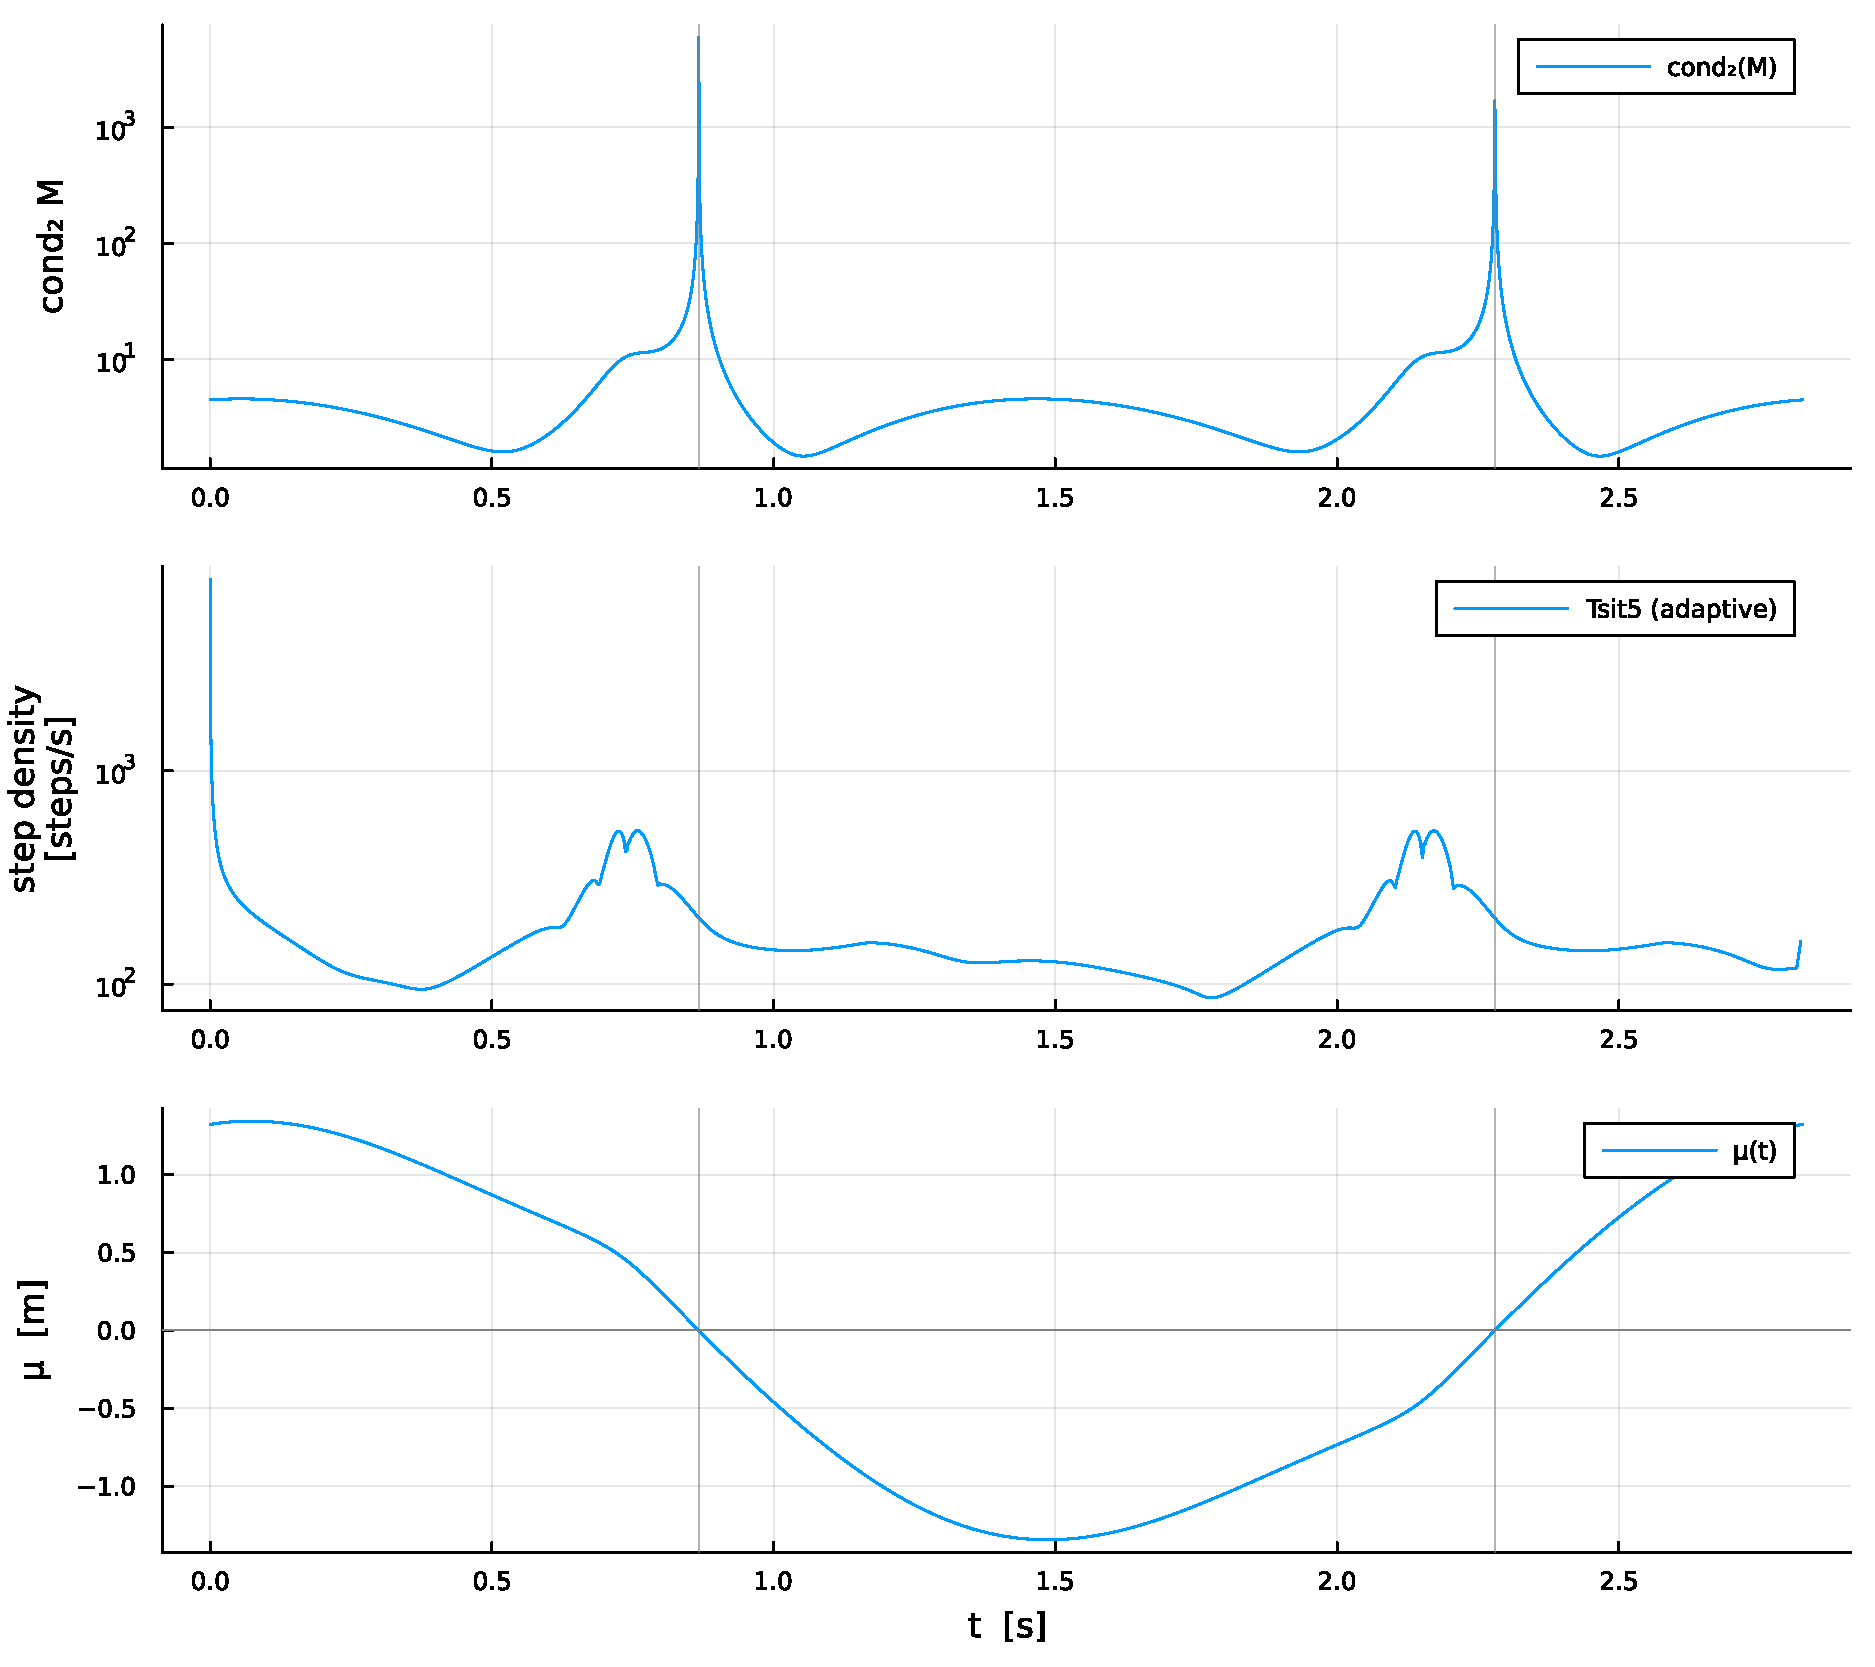
\includegraphics[width=0.95\textwidth]{figs/conditioning.pdf}
    \caption{One limit cycle with $\dot\tau > 0$ (period
    $T \approx 2.8$\,s): condition number of $M$ (top), accepted-step
    density of the adaptive \texttt{Tsit5} integrator
    ($\mathrm{tol} = 10^{-10}$, middle) and lever arm $\mu$ (bottom),
    on a common time axis; gray lines mark the zeros of $\mu$
    ($\phi = \alpha$).  Both the conditioning spikes and the density
    humps line up with the crossings (the $t = 0$ density spike is a
    start-up artifact).}
    \label{fig:conditioning}
\end{figure}
\begin{figure}[htbp]
    \centering
    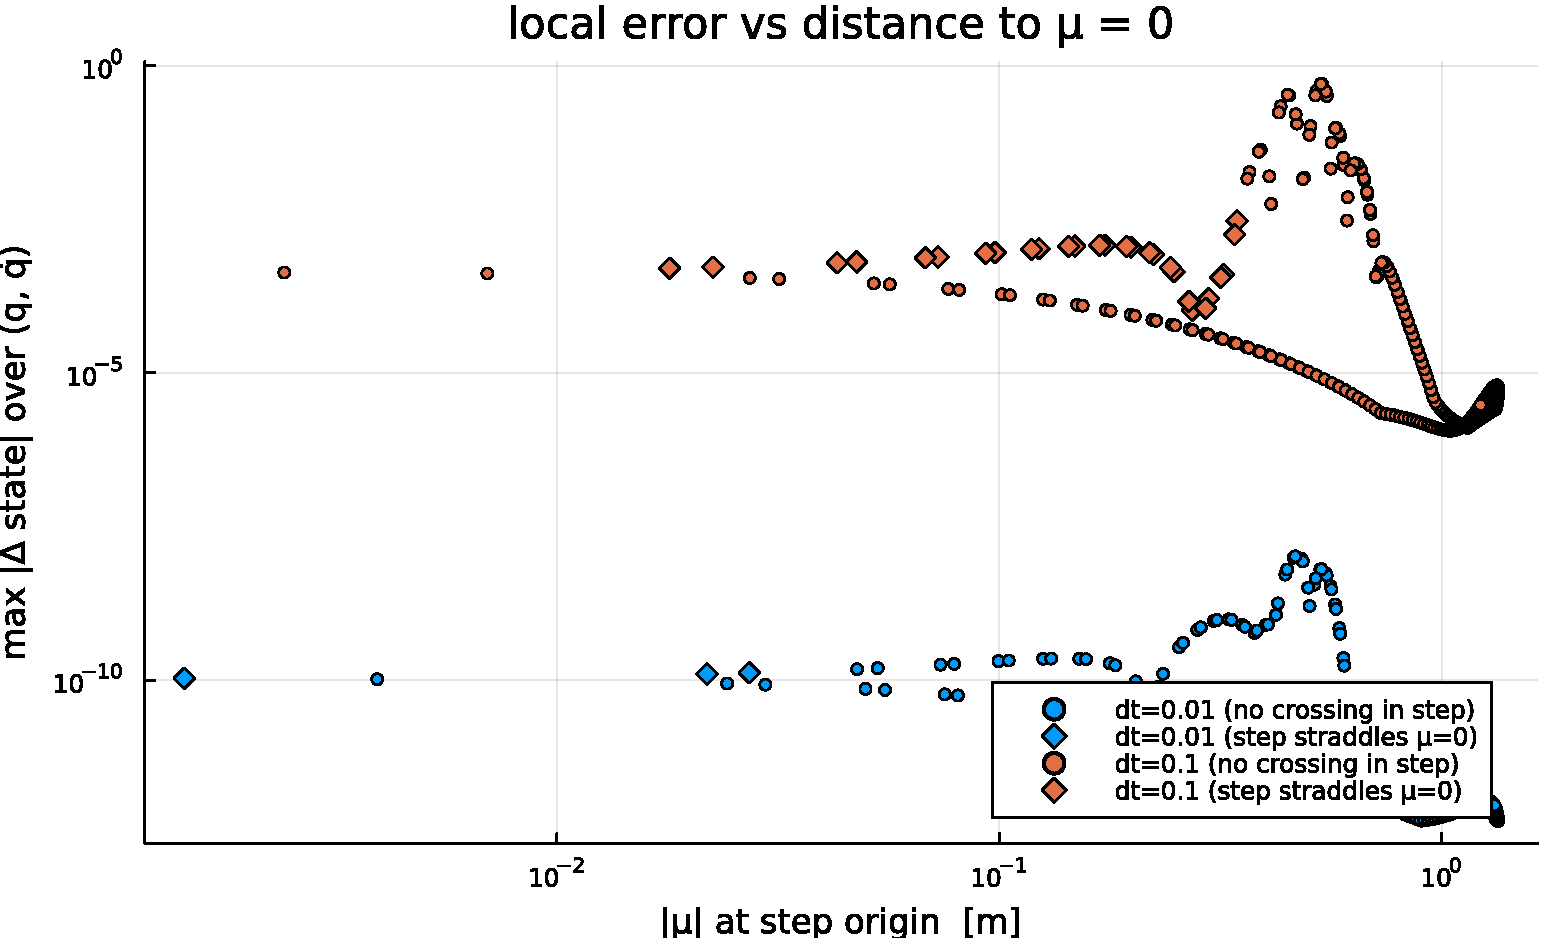
\includegraphics[width=0.7\textwidth]{figs/local_error.pdf}
    \caption{Local error of a single fixed-size \texttt{Tsit5} step
    ($\delta t = 10^{-2}$\,s, the adaptive integrator's operating scale,
    and $0.1$\,s, an order of magnitude beyond its largest accepted
    step), each measured against a fresh $10^{-13}$-tolerance solve of
    the same step, plotted against $\lvert\mu\rvert$ at the step origin;
    diamonds mark steps that straddle a $\mu = 0$ crossing.  The
    committed error never diverges as the singular set is approached,
    and the crossing premium shrinks to the integration tolerance at the
    integrator's own step sizes.}
    \label{fig:local-error}
\end{figure}

Equation \eqref{eq:ddq-final} closes the derivation: it delivers the
accelerations $\ddq = F(\vq, \dq)$ explicitly, so the model is a pure
second-order \gls{ode} on $\vq \in \R^2$ whose integration needs neither a
symbolic solver nor the manifold-projection callback of the five-state
formulation.

\appendix
\section{The five-state formulation for comparison}
\label{sec:model10D}

The reference five-state model describes the same system with five
configuration variables
\begin{equation} \label{eq:state_vector_10D}
    \vq_{10} = (\alpha, \theta_\ell, \phi_\ell, r, \tau)
    \in \R^5
\end{equation}
subject to the three algebraic loop-closure constraints
$\vb g(\vq_{10}) = 0_{\R^3}$, i.e.\ a \gls{dae} with two \gls{dof}.  Its
reduction requires index reduction (two differentiations of the
constraints), a symbolic solver for the implicit accelerations, consistent
initial conditions satisfying six scalar relations, and---in
practice---a manifold-projection callback to prevent drift of $\vb g$ and
$\dot{\vb g}$.  Formula \eqref{eq:ddq-final} is the same physics in the
minimal coordinates: the loop constraint is solved once and for all for
$r(\alpha, \tau)$, the cone is built into the coordinates, and the two
remaining acceleration equations are inverted by hand.

\end{document}
